\writtenby{\dcauthornameriren}%
In diesem Teilbereich der Evaluation wird die Bibliothek ZXing auf ihren Funktionsumfang getestet.
Verschiedene Strichcodearten werden normal, unscharf, verdunkelt, rotiert und schattiert der Bibliothek übergeben und es wird überprüft, bis zu welchem Grad die Codes trotzdem erkannt werden.

Dabei sind die Tests auf den Strichcode EAN-13 und den in 2D aufgebauten QR-Code beschränkt, da diese repräsentative Mengen bilden. Denn Strichcodes sind im Grunde alle ähnlich aufgebaut (siehe Figur \ref*{fig:similarcodes}) und haben nur eine andere Codierung oder vereinzelt Überprüfungsmechanismen, sind aber sonst gleicher Art und haben die gleichen Schwächen. Der QR-Code ist dafür der am meisten verwendete 2D Code (etwa 88\% in 2011) und alle anderen werden kaum bzw. nur in Spezialfällen benutzt, wie es aus einer Studie von Competitrack im Jahre 2011 über 2D Codes in der Werbung hervor geht.
\todo{QUELLE}

\begin{figure}[H]
  \centering
  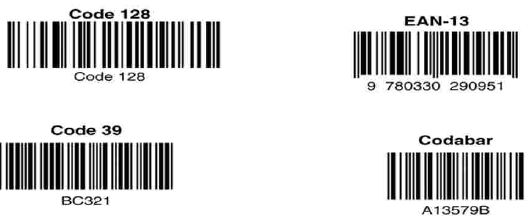
\includegraphics[height=5cm]{img/EAN13/strichcodes.jpg}
  \caption{Verschiedene Strichcodes, weisen trotzdem die gleichen Eigenschaften auf.}
  \label{fig:similarcodes}
\end{figure}

Die Ergebnisse sind empirisch getestet worden und ergeben einen guten Überblick über die Möglichkeiten und Einschränkungen der Strichcodeerkennung durch die ZXing Bibliothek. Die verwendeten Beispielcodes wurden durchgängig genutzt, um direkt die Unterschiede in der Erkennung sichtbar machen zu können. Die zugrunde liegenden Codes werden dabei in den Figuren \ref*{fig:eannormal} (1. und 2. Bild) und \ref*{fig:qrnormal} (1. und 3. Bild) dargestellt.
